\documentclass[11pt, A4paper, english]{article}
\usepackage[utf8]{inputenc}
\usepackage[T1]{fontenc}
\usepackage{babel}
\usepackage{amsmath}
\usepackage{amsfonts}
\usepackage{amsthm}
\usepackage[colorlinks]{hyperref}
\usepackage{listings}
\usepackage{color}
\usepackage{hyperref}
\usepackage{graphicx}
\usepackage{cite}
\usepackage{float}
\usepackage{multicol}

\definecolor{dkgreen}{rgb}{0,0.6,0}
\definecolor{gray}{rgb}{0.5,0.5,0.5}
\definecolor{daynineyellow}{rgb}{1.0,0.655,0.102}
\definecolor{url}{rgb}{0.1,0.1,0.4}

\lstset{
frame=tb,
language=Python,
aboveskip=3mm,
belowskip=3mm,
showstringspaces=false,
columns=flexible,
basicstyle={\small\ttfamily},
numbers=none,
numberstyle=\tiny\color{gray},
keywordstyle=\color{blue},
commentstyle=\color{daynineyellow},
stringstyle=\color{dkgreen},
breaklines=true,
breakatwhitespace=true,
tabsize=3
}

\lstset{inputpath="C:/Users/Torstein/Documents/UiO/Ast2210/Python programmer"}
\graphicspath{{C:/Users/Torstein/Documents/UiO/Ast2210/"Python programmer"/}}
\hypersetup{colorlinks, urlcolor=url}

%\lstinputlisting{Filnavn! type kodefil}
%\includegraphics[width=12.6cm,height=8cm]{Filnavn! type png}


\author{Torstein Solheim Ølberg \\
Institute for Theoretical Astrophysics, University of Oslo \\
P.O. Box 1029 Blindern 0315 Oslo, Norway}
\title{Learning about light behaviour and the JWST}

\begin{document}

\maketitle

	\section{Abstract}
In this report we are going to look at the behaviour of light and how that limits the resolution of our telescopes. We start by pointing a at a slit and getting a diffraction pattern, then we set up a camera and record a laser through a microscopic objective, a lens and an aperture. Here we got an Airy disk and when switching the setup for a coin we saw a bright dot in the centre of a dark spot. Then we calculated the constant $K$ for a formula and used this formula to estimate size resolutions for JWST, wich turnd out to be quite good, thought not good enough to spy on humans very much.

	\begin{multicols}{2}
		\section{Introduction}
In astrophysics it is important to know of the properties of light, especially its wavelike characteristics, as these have a critical influence on our ability to measure, and collect information from different events. Because of this I want to try to learn a bit more about lights behaviour. Especially about how it influences the angular resolution, as this is important to estimate how good a telescope will be. What I want to do then is to be able to calculate slit widths and wavelengths, and also estimate a formula for the angle of the minimums on an image of light through a hole. At the end I will try to use this information to estimate the angular resolution of the JWST and also estimate the size of objects JWST can resolve at different distances to the telescope. \\
To begin with we assume the gravity doesn't effect the light, and that all of the experiments are conducted in a system at constant velocity. Later, when estimating the characteristics of JWST's we will assume that JWST is positioned in first near-Earth orbit, then on the Earth, in our solar system and in the end in our Galaxy. This is because the difference between the real position of the telescope compared to the assumed position is negligible with respect to the actual distance to the object we are interested in resolving.  We will also assume that the distance $\sin(\theta)$ in the formula
$$\sin(\theta) = \frac{K \lambda}{d}$$
is so small it is approximately equal to $\theta$. \\
To be able to get the results in this report I will need to know of the diffraction equations
$$a \sin(\theta) = m \lambda$$
$$\sin( \theta) = \frac{K \lambda}{d}$$
and to be able to combine these with the definition of sinus
$$\sin(\theta) = \frac{D}{L}$$
I need to know that the $K$ value for the second minimum is $2.23$ \cite{labinstruks}. I also need Babinet's Principle, which states that the diffraction pattern from a slit and the complementary anti-slit on the same spot is the same as if none of them where there \cite{Babinet}. This means that an object will produce a diffraction pattern just like if it was a slit, but the maximums and minimums will switch places. Then in the end i need the diameter $d \approx 6 m$ and the observable frequency interval $f = (600 nm - 28.5 \mu m)$ of JWST \cite{JWST}, the distance form near-Earth orbit to the ground $L_{orb} \approx 540 km$ \cite{labinstruks}, the distance from Earth to the sun $L_{sun} = 1 AU \approx 150 Gm$ \cite{SunEarth}, the distance from the solar system to our galaxy's centre $L_{Gc} \approx 8 kpc = 246 Zm$ \cite{GalaCenter} and how much $4$ billion light years are in meters.


		\section{Equipment}
			\begin{itemize}
\item A small laser with some visible light
\item A platform to hold the laser
\item A $100 \mu m$ slit in a stand
\item A paperclip on a stand
\item A white sheet of paper and a pencil
\item A wall or other background to point the laser at (Should not be easily movable)
\item A laser fitted on a collimator tube with a dampening filter
\item A $f = 100 mm$ doublet lens and an adjustable stand for it
\item A microscope objective on an adjustable stand which magnifies $20$ times
\item A Mono-chromatic camera on an adjustable stand with $6 \mu m$ pixels
\item A computer with software for taking and viewing pictures with the camera
\item A coin without a central hole
			\end{itemize}


		\section{Methods}
First we mounted the laser on the stand an align it to point through the slit and hit the wall behind. Then we put a paper on the wall and used the pencil to mark the diffraction pattern from the laser, starting on the nr. $1$ maximum and marked the pattern to the right of it. Then we measured the distance between the slit and the wall and the distance between the first maximum and the twelfth minimum. With this we calculated the wavelength of the light through the equation $\lambda = \frac{a \sin(\theta)}{m}$, where a is the slit width, $\theta$ is the angle between the minima and the first maximum and $m$ is the order of the minimum We obtain the sinus of the angle $\theta$ by taking the distance between the first maximum and the twelfth minimum, $D$, divided by the distance $L$ between the slit and the wall. Thus the equation becomes
$$\lambda = \frac{a D}{Lm}$$
\\
Then we replaced the slit with a paperclip, bent such that it has a straight metal piece, and pointed the laser on it. Now we needed to move the paperclip longer from the wall than the slit was, since the clip is much wider than the slit. Then we recorded the diffraction pattern in the same way as before and measured the same distances, except that we used the first minimum and the $25$th maximum this time. In the end we used the equation
$$a = \frac{\lambda L m}{D}$$
and found the width of the paperclip.
\\
Now, having done that we switched to another set-up. Now we used a laser connected to a collimator tube, a doublet, $100 m$, lens, a microscope objective and a mono-chromatic camera. We used the piece of paper to set up the different items along a parallel line, where the lens is placed first such that the light from the laser is centred on the lens, the objective is placed in the focal point of the lens and the camera right behind the objective. Then we put the filter between the laser and the collimator tube and started our program to record the light that the camera records. Now we saw a bright Airy pattern. With this set-up took a picture of the pattern, and counted the amount of pixels on the picture between the first maximum and the first and second minimum. Then we used the formula 
$$d = \frac{K \lambda L}{D}$$
where $d$ is the diameter of the aperture, $K$ is the constant dependant of which minimum we are looking at, $\lambda$ is the wavelength of the light used, $L$ is the distance between the lens and the camera and $D$ is the distance form the centre maximum to the minimum we are looking at. After this we took an exposure of the dust on the optical system. Then we switched out the lens with a coin and removed dampening filter, the camera and the objective, and pointed the laser and coin on the wall behind. As we now had estimated a formula for the resolution of a telescope with the diameter $d$, we could use this to estimate the resolution of JWST, first when looking at earth, then the sun, then the Milky Way's centre and last of all a hypothetical galaxy $4$ billion light years away.
	\end{multicols}

		\section{Results}
			\begin{tabular}{|l|r|}
\hline
Measured & Data \\
\hline
Distance slit, wall & $120.7(3) cm$ \\
Distance maximum nr. $1$, minimum nr. $12$ & $9.0(2) cm$ \\
Distance paperclip, wall & $195.8(10) cm$ \\
Distance minimum nr. $1$, maximum nr. $25$ & $3.5(1) cm$ \\
Pixels from centre to minimum nr. 2 & $8.5(5) \text{pixels}$ \\
Pixels from centre to minimum nr. 1 & $6.5(5) \text{pixels}$ \\
\hline
			\end{tabular}
			\begin{figure}[H]
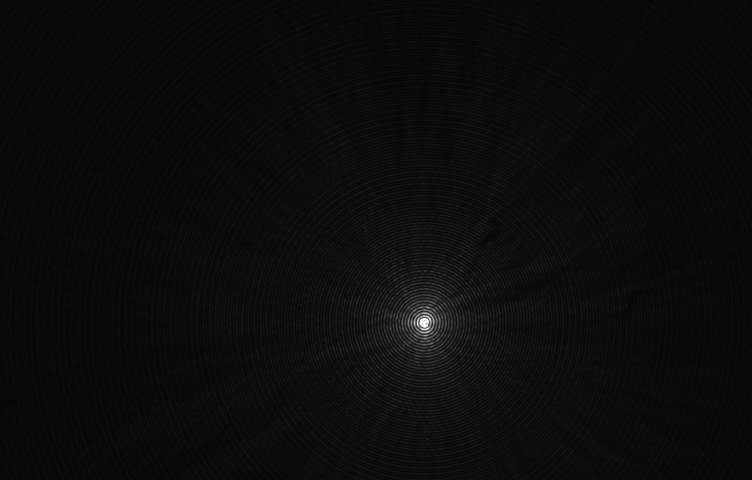
\includegraphics[width=12.6cm, height=8cm]{Lab1Airy.png}
\caption{Exposure of Airy disk from objective microscope}
			\end{figure}
			\begin{figure}[H]
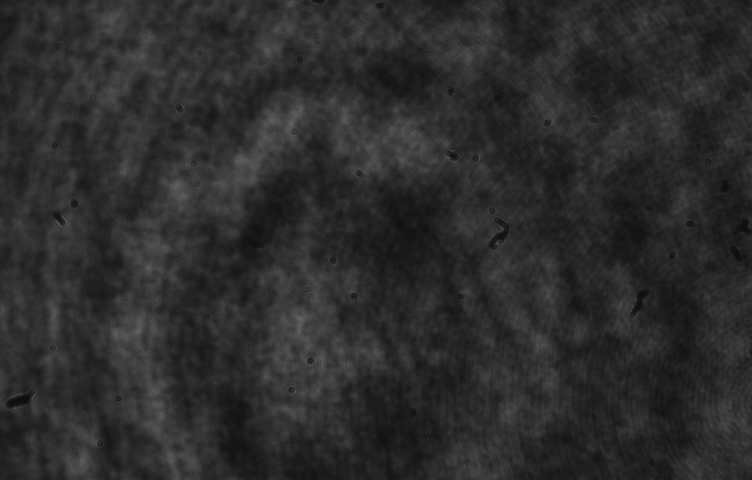
\includegraphics[width=12.6cm, height=8cm]{Lab1Dust.png}
\caption{Exposure of dust for the setup without objective}
			\end{figure}
When looking at the pattern from the coin we saw a small weak spot in the middle of the dark area.
	\begin{multicols}{2}
		\section{Conclusion/Discussion}
From the results of the slit experiment we get that the wavelength of the light from the laser is
$$\lambda = \frac{a D}{L m}$$
$$\lambda = \frac{100 \mu m \cdot 9.0(2) cm}{120.7(3) cm \cdot  12} = 621(30) nm$$
where the uncertainty is estimated from our measurements on the spot and comes from our own ability to measure and what we used to measure with. We can see that the resulting wavelength is in the red spectrum of the visible light, which is what we would expect since we could se the laser light and it was red.
Then we can find that the width of the paperclip is
$$a = \frac{\lambda L m}{D}$$
$$a = \frac{621(30) nm \cdot 195.8(10) cm \cdot 25}{3.5(1) cm}$$
$$ \lambda = 0.87(10) mm$$
\\
As for the Airy disk we can now get the diameter of the aperture with
$$d = \frac{K \lambda L}{D}$$
$$d = \frac{2.23 \cdot 621(30) nm \cdot 0.1 m \cdot 20}{8.5(5) \cdot 6 \mu m}$$
$$d = 0.054(5) m$$
And using this we get that for the first minimum
$$K = \frac{d D}{\lambda L}$$
$$K = \frac{0.054(5) m \cdot 6.5(5) \cdot 6 \mu m}{621(30) nm \cdot 0.1 m \cdot 20} = 1.7(5)$$
which is smaller than for the second minimum, just as you would expect. Now we took a look at the dust patterns, and as you can see on the exposure there are small lighter lines along the rim of the dust patterns. These come from the dust obscuring the light and acting as small anti-lenses, bending the light. This is even more obvious in the next part where we switched out the lens for a coin. Here we could see that there was a small, weak spot in the middle of the dark spot, resulting from the coin working as an anti-lens, focusing the light to a single spot. \\
\\
Finally we have the estimates for JWST. Here we use the formula
$$\theta_{\text{min}} = \frac{K \lambda}{d}$$
getting that the angular resolution of JWST for $600 nm$ and $28.5 \mu m$ is
$$\theta_{\text{min}} = \frac{1.7(5) \cdot 600 nm}{6 m} = 0.000612(50)''$$
$$\theta_{\text{min}} = \frac{1.7(5) \cdot 28.5 \mu m}{6 m} = 0.0291(50)''$$
To get the physical size of an object JWST can resolve, we use that $\theta_{\text{min}} \approx \sin(\theta) = \frac{D}{L}$. That means the size is given by
$$D = L \theta_{\text{min}}$$
and we get these results for different distances.
	\end{multicols}
	\begin{tabular}{|l|c|r|}
\hline
JWST pointed at & Resolution $600 nm$ & Resolution $28.5 \mu m$ \\
\hline
Earth & $0.0918(50) m$ & $4.365(500) m$ \\
Sun & $25.5(50) km$ & $1212.5(5000) km$ \\
Galactic centre of Milky Way & $4.128(500) \cdot 10^{13} km$ & $1.9885(5000) \cdot 10^{15} km$ \\
Galaxy $4$ Giga light years away & $6.4328(5000) \cdot 10^{15} km$ & $3.05873 \cdot 10^{17} km$ \\
\hline
	\end{tabular}
	\begin{multicols}{2}
The reason i have choose to include the Earth as a target is for the few people out there wondering if JWST will be able to spy on us for the government, and as you can see. you will have to write quit big letters if they are going to be recognizable when the resolution is $9 cm$. As for the other results, the Sun is a lot larger than resolution here, almost half million km in diameter, if I am not to of and you will be able to se a good bit of detail on its surface. The super massiv black hole in the centre of the Milky Way is a few billion km in diameter I believe, so we will not be able to resolve it so well, but other galaxies are typically around the resolution size of JWST at 4 billion light years away I think so we should be able to see them ok.
\addcontentsline{toc}{chapter}{Bibliography}
		\begin{thebibliography}{9}
			\bibitem{labinstruks}
Souvik Bose; \\
AST2210 - Lab exercise: Diffraction and angular resolution \\
\url{http://folk.uio.no/hke/AST2210/diffr_lab.pdf} \\
Downloaded 23/09-2018
			\bibitem{Babinet}
Zhong Ming Tan; Kirk T. McDonald; \\
Babinet’s Principle for Electromagnetic Fields \\
\url{http://www.hep.princeton.edu/~mcdonald/examples/babinet.pdf} \\
Downloaded 23/09-2018
			\bibitem{JWST}
NASA; \\
Webb Vital Facts \\
\url{https://jwst.nasa.gov/facts.html} \\
Downloaded 23/09-2018
			\bibitem{SunEarth}
NASA; \\
Measuring the Distance \\
\url{https://www.nasa.gov/audience/foreducators/k-4/features/F_Measuring_the_Distance_Student_Pages.html} \\
Downloaded 23/09-2018
			\bibitem{GalaCenter}
NASA; \\
Imagine The Universe! \\
\url{https://imagine.gsfc.nasa.gov/features/cosmic/milkyway_info.html} \\
Downloaded 23/09-2018
		\end{thebibliography}
	\end{multicols}
\end{document}